%================================================================
\chapter{Supervised Learning}\label{chap:SupervisedLearning}
%================================================================

This chapter introduces the fundamentals of supervised learning, optimization and neural networks. The content of this chapter is mainly based on the material in \citet{SupervisedwquantumComputers}, \citet{hastie01statisticallearning} and \citet{nielsenneural}.

The goal of \emph{supervised learning}, one of the big branches of machine learning, is to obtain a model for predicting an output $y$ from an input $\boldsymbol{x}$. This is done by learning from input-output pairs $\mathcal{T} = \{(\boldsymbol{x}^{(1)}, y^{(1)}), \cdots, (\boldsymbol{x}^{(N)}, y^{(N)})\}$, known as the training set. Here, we assume that $\boldsymbol{x}^{(i)}$ is a vector and $y$ is a scalar. The domain of the input and output depends on the specific learning problem. The output $y$, also called the target or the response, is often either of a quantitative or qualitative character. These two cases constitute two big paradigms in supervised learning: \emph{regression} and \emph{classification}, respectively. For regression, the goal of the learning task is to predict a real-valued target y from the input $\boldsymbol{x}$. Typical examples of targets to regress on are \emph{temperature}, \emph{weight} and \emph{length}, which have in common a natural notion of distance measure in the sense that instances close in numerical value are also similar in nature. E.g., two fish weighing $12.1$ kg and $12.2$ kg are similar, while a third fish weighing $24.0$kg is notably different.

For classification, the goal is to predict one or more \emph{classes} from an input $\boldsymbol{x}$. In this setting, the target $y$ is discrete and categorical, such as \emph{color}, \emph{dead/alive} and \emph{animal species}. In contrast to quantitative targets, qualitative targets lack a natural distance measure, in the sense that it is not meaningful to compare the distance between \emph{dog} and \emph{cat}, and \emph{dog} and \emph{seagull}. They are simply mutually exclusive classes.

The input $\boldsymbol{x}$ is a vector consisting of elements $(x_1, \cdots, x_p)$ often called features or predictors. Each feature $x_i$ can either be quantitative or qualitative in the same manner as with the target previously discussed. In this thesis, we will investigate quantitative features $\boldsymbol{x} \in \mathbb{R}^{p}$.


%================================================================
\section{Parametric Models}\label{sec:ParametricModels}
%================================================================
The approach of supervised learning often starts by acquiring a training set $\mathcal{T} = \{(\boldsymbol{x}^{(1)}, y^{(1)}), \cdots, (\boldsymbol{x}^{(N)}, y^{(N)})\}$, where $N$ is the number of samples in the training set. This is called labeled data, since the samples of features $\boldsymbol{x}^{(i)}$ are accompanied by the ground truth target $y^{(i)}$  that we want to predict. One often hypothesizes that the acquired training data was produced by some mechanism or process that we can mathematically express as

\begin{equation}\label{eq:data}
    y = \hatf(\boldsymbol{x}) + \epsilon,
\end{equation}
where $\epsilon$ is often included to account for randomness, noise or errors in the data, in contrast to the deterministic part $f(\boldsymbol{x})$. Depending on the context, the $\epsilon$ may be neglected or assumed to be normally distributed such as $\epsilon \sim \mathcal{N}(0, \sigma^2)$, where $\sigma^2$ is the variance.

The goal is to approximate the underlying mechanism $f(\boldsymbol{x})$. To do this, one often proposes a parametric model

\begin{equation*}
    \hat{y} = \hat{f}(\boldsymbol{x}; \boldsymbol{\theta}),
\end{equation*}

where $\hat{y}$ is the predicted value, $\hat{f}(\cdot; \cdot)$ defines a family of models, and $\boldsymbol{\theta}$ is a vector of parameters that defines a specific model from that family. Training (or fitting) the model involves finding the parameters $\boldsymbol{\theta}$ such that the model best reproduces the targets from the features found in the training data set. To quantify what is meant by "best" in this context, it is common to introduce a \emph{loss function} that measures the quality of the model with respect to the training data set:

\begin{equation}\label{eq:LossFunction}
    L(\boldsymbol{\theta}) = \frac{1}{N}\sum_{i=1}^{N} L(\hat{f}(\boldsymbol{x}^{(i)}; \boldsymbol{\theta}) , y^{(i)}),
\end{equation}

The loss function returns a scalar value that indicates how good your model fits the training data for a particular set of parameters. In general, a lower value indicates a better model. This formulates the task of training the model as an optimization problem. In the next section, we will discuss different ways of training parameterized models, in particular with the use of gradient-based methods.

%================================================================
\subsection{Regression}\label{sec:Regression}
%================================================================

The choice of loss function is highly problem dependent, and there is a vast collection of different choices in the machine learning literature \cite{hastie01statisticallearning}. A common loss function used for training supervised models on regression problems is the Mean Squared Error (MSE). This loss function is suitable since it implements a natural distance measure between prediction and target. It is formulated as

\begin{equation}\label{eq:MSE}
    MSE = \frac{1}{N}\sum_{i=1}^{N} (\hat{f}(\boldsymbol{x}^{(i)}; \boldsymbol{\theta}) - y^{(i)})^2.
\end{equation}

From this formulation, we see that the closer the predicted targets $\hat{y}^{(i)} = \hat{f}(\boldsymbol{x}^{(i)}; \boldsymbol{\theta})$ are to the real targets $y^{(i)}$, the smaller the MSE will be. In other words, a model with lower MSE than some other model fits the data better. Fitting the model using MSE as loss function is often referred to as the \emph{least squares approach}.

%================================================================
\subsection{Classification}\label{sec:Classifcation}
%================================================================
In this thesis, we will be concerned with \emph{binary classification}, where the targets of the data are one of two classes that we want to predict. Typically, the different classes are represented by discrete values, such as $y \in \{0,1\}$. Here $0$ and $1$ corresponds to the first and second class, respectively. When parametric models are trained on discrete targets, by for example by minimizing the MSE loss, they tend to produce output values in the range $\hat{f}(\boldsymbol{x}^{(i)}; \boldsymbol{\theta}) \in [0,1]$. The continuous value of $\hat{f}(\boldsymbol{x}^{(i)}; \boldsymbol{\theta})$ are often interpreted as the probability that sample $\boldsymbol{x}^{(i)}$ belongs to the second class. As an example, say $f(\boldsymbol{x}^{(i)}; \boldsymbol{\theta}) = 0.8$ for a particular sample $\boldsymbol{x}^{(i)}$. This tells us that it belongs to the second class with $80\%$ probability, and to class $0$ with $20\%$ probability. A class can then be predicted from the sample by implementing a \emph{threshold value} $c$, such as
\begin{equation}
    \hat{y}^{(i)} = I(f(\boldsymbol{x}^{(i)}; \boldsymbol{\theta}) > c),
\end{equation}
where $I()$ returns one if $f(\boldsymbol{x}^{(i)}; \boldsymbol{\theta}) > c$ is true, and otherwise zero. Typically, a threshold value $c = 0.5$ is used, as this causes the most probable class to be picked  

Whereas MSE can be used to assess how closely regression models fits the data, a more suitable metric for assessing classification models is \emph{accuracy}. The accuracy can be expressed as 

\begin{equation}\label{eq:accuracy}
    \text{accuracy} = \frac{1}{N}\sum_{i=1}^{N} I(\hat{y}^{(i)} = y^{(i)}).
\end{equation}

From \cref{eq:accuracy}, we see that the accuracy of a model is the average number of targets it classifies correctly.  


%================================================================
\section{Optimization}\label{sec:Optimization}
%================================================================
Finding the optimal parameters $\hat{\boldsymbol{\theta}}$ with respect to a chosen loss function $L$ can be formulated as

\begin{equation}\label{eq:Optimization}
    \hat{\boldsymbol{\theta}} = \underset{\boldsymbol{\theta}}{\argmin} \frac{1}{N}\sum_{i=1}^{N} L(f(\boldsymbol{x}^{(i)}; \boldsymbol{\theta}) , y^{(i)}).
\end{equation}

This optimization problem is generally not trivial, and depends highly on the choice of loss function and parametric model. Aside from a few exceptions, like the case of linear regression, \cref{eq:Optimization} does not generally have an analytical solution. Moreover, many popular parametric models result in non-convex optimization problems, meaning that the loss function has several local minima. In practice, such optimization problems can't be solved efficiently \cite{Vava:book}. However, it is important to realize that an exact, or close to exact, minimization of the loss function is seldom needed or even favorable. What is ultimately interesting is whether the trained model has sufficient ability to predict. Over the years, several cheap and approximate methods for optimization have been invented to train machine learning models. We will discuss two such methods that implement gradient-based optimization. 

%================================================================
%\subsection{Matrix Inversion}\label{sec:MatrixInvertion}
%================================================================
%(uferdig avsnitt, skal kanskje droppes)
%Linear regression models are defined as 

%\begin{equation*}
%    f(\boldsymbol{x}; \boldsymbol{\beta}) = \sum_{j=0}^p x_j \beta_j =  \boldsymbol{x}^T %\boldsymbol{\beta},
%\end{equation*}
%where $\boldsymbol{x}^T = [1, x_1, \cdots, x_p]$ is a vector of $p$ features together with a constant $1$ %to account for the intercept of the model, and $\boldsymbol{\beta}$ is a vector of model parameters %called coefficients. Using least squares approach leads to the following loss function:

%\begin{equation*}
%    L(\boldsymbol{\theta}) = \frac{1}{N}\sum_{i=1}^{N} (\sum_{j=0}^p x_j^{(i)} \beta_j -  y^{(i)})^2.
%\end{equation*}

%This objective function can be reformulated using matrix and vector notation as

%\begin{equation*}
%    L(\boldsymbol{\theta}) = (\boldsymbol{X}\boldsymbol{\beta} - %\boldsymbol{Y})^T(\boldsymbol{X}\boldsymbol{\beta} - \boldsymbol{Y}),
%\end{equation*}
%where $\boldsymbol{X}^T = [\boldsymbol{x^}]$ 

%================================================================
\subsection{Batch Gradient Descent}\label{sec:GradientDescent}
%================================================================
In the absence of an analytical expression that minimizes the loss function, \emph{gradient descent} is an easy-to-implement method that iteratively decreases the loss. This is done by repeatedly adjusting the model parameters using information of the \emph{gradient} of the loss function. The derivative of the loss function \cref{eq:LossFunction} with respect to the model parameters can be calculated as

\begin{equation}\label{eq:LossDerivateWRTparameter}
    \frac{\partial L(\boldsymbol{\theta})}{\partial \theta_k}  =
    \frac{1}{N}\sum_{i=1}^{N} \frac{\partial L( \hat{y}^{(i)}, y^{(i)})}{\partial \hat{y}^{(i)}} 
    \frac{\partial \hat{y}^{(i)}}{\partial \theta_k},
\end{equation}
where $\theta_k$ is the $k$'th model parameter, and  $\hat{y}^{(i)} = \hat{f}(\boldsymbol{x}^{(i)}; \boldsymbol{\theta})$. To arrive at this expression, the chain rule was used under the assumption that the loss function $L(\hat{y}^{(i)}, y^{(i)})$ and model output $\hat{y}^{(i)}$ are differentiable with respect to $\hat{y}^{(i)}$ and $\theta_k$, respectively. For MSE loss \cref{eq:MSE}, the derivative has the form 

\begin{equation}\label{eq:LossDerivateWRTparameter}
    \frac{\partial L(\boldsymbol{\theta})}{\partial \theta_k}  =
    \frac{2}{N}\sum_{i=1}^{N} (\hat{y}^{(i)} - y^{(i)}) 
    \frac{\partial \hat{y}^{(i)}}{\partial \theta_k}.
\end{equation}

Note that the derivative is calculated with respect to the entire training set, i.e. the whole \emph{batch}, hence the name. The gradient is then constructed simply as a vector quantity containing the derivatives with respect to each model parameter:

\begin{equation}\label{eq:Gradient}
    \nabla_{\boldsymbol{\theta}} L(\boldsymbol{\theta})= 
    \big{(} \frac{\partial}{\partial \theta_1} L(\boldsymbol{\theta}), 
    \cdots, \frac{\partial}{\partial \theta_{n_{\theta}}} L(\boldsymbol{\theta}) \big{)},
\end{equation}
where $n_{\theta}$ is the number of parameters. The gradient \cref{eq:Gradient} can be geometrically interpreted as the direction at point $\boldsymbol{\theta}$ in parameter space for which the value of the loss function increases most rapidly. In light of this, one can attempt to move all the parameters some small amount in the opposite direction, \emph{the direction of steepest descent}, in order to decrease the loss. This can be done iteratively, and can be formulated as 


\begin{equation}\label{eq:ParameterUpdate}
    \boldsymbol{\theta}_{t} = \boldsymbol{\theta}_{t-1} - \mu \nabla_{\boldsymbol{\theta}} L(\boldsymbol{\theta}_{t-1})
\end{equation}
for $t=1, \cdots, T$. Here, $T$ is the total number of  iterations, or \emph{epochs}, and $\mu$ is some small positive value called the \emph{learning rate}. Usually, some initial choice of parameters $\boldsymbol{\theta}_{0}$ is chosen at random. Analogous to walking down a mountain, the recalculation of the gradient and repeated adjustment of the parameters results in a gradual descent in the loss landscape. This is the heart of gradient descent.

Even though batch gradient descent is intuitively simple and sometimes sufficiently effective for training some models, it has several flaws that should be addressed when suggesting better methods of optimization. A common problem with batch gradient descent is that optimization has a tendency of getting stuck in local minima, as only local information in the loss landscape is used when updating the parameters. In addition, the presence of \emph{plateaus}, areas of particular flatness in the loss landscape, tend to induce slow convergence. The two aforementioned phenomena are illustrated in \cref{fig:localMinima}.  


\begin{figure}[htp]
    \centering
    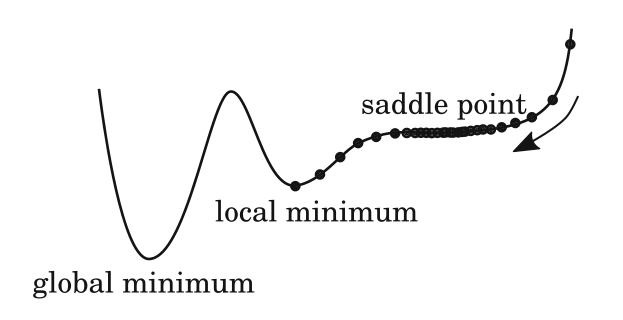
\includegraphics[width=10cm]{latex/figures/local_minimum_saddle_point.png}
    \caption{One-dimensional representation of the loss landscape for a parameterized model, showcasing the phenomenon of getting stuck in local minima, and slow convergence induced by plateaus. The figure is retrieved from \citet{hands-on}.}
    \label{fig:localMinima}
\end{figure}

Furthermore, the presence of high degree of distortion in certain directions in parameter space, so called  \emph{thin valleys}, can lead to oscillations and inefficient optimization. This is exemplified in \cref{fig:thinValley}. We will discuss how the popular \emph{Adam optimizer} \cite{kingma2017adam}, which was used in this thesis, addresses these problems.

\begin{figure}[htp]
    \centering
    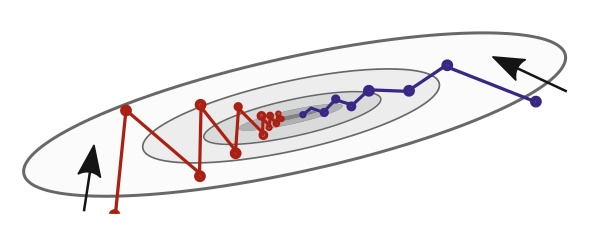
\includegraphics[width=10cm]{latex/figures/thin_vally.png}
    \caption{Two-dimensional representation of the loss landscape for a parameterized model, showcasing the phenomenon of "thin valleys", known to induce slow convergence due to oscillations. The blue optimizations steps incorporate momentum, which dampens the oscillations and leads to faster convergence. The figure is retrieved from \citet{SupervisedwquantumComputers}.}
    \label{fig:thinValley}
\end{figure}



%================================================================
\subsection{Adam Optimizer}\label{sec:AdamOptimizer}
%================================================================
Introduced by \citet{kingma2017adam}, the Adam algorithm implements a moving average of the gradient, called \emph{momentum}, together with a rescaling. Replacing \cref{eq:Gradient} and \cref{eq:ParameterUpdate}, Adam implements the following algorithm:

\begin{algorithm}[H]
\caption{\emph{Adam}, \cite{kingma2017adam}. The authors suggest default hyperparameters $\alpha = 0.001$, $\beta_1 = 0.9$, $\beta_2 = 0.999$ and $\epsilon = 10^{-8}$. The algorithm is applied parameter-wise.}
\label{alg:Adam}
\SetAlgoLined

$m_0 \gets 0$;\\
$v_0 \gets 0$;\\
$t \gets 0$;\\
\While{$\theta_t$ not converged}{
$t$ \gets $t+1$\\
$g_t \gets \nabla_{\theta} L(\theta_{t-1})$
(Get gradients w.r.t. loss at timestep $t$)\\
$m_t \gets \beta_1 m_{t-1} + (1-\beta_1) g_{t}$
(Update biased first moment estimate)\\
$v_t \gets \beta_2 v_{t-1} + (1-\beta_2) g_{t}^2$
(Update biased second raw moment estimate)\\
$\hat{m}_t \gets m_t/(1 - \beta_1^{t})$
(Compute bias-corrected first moment estimate)\\
$\hat{v}_t \gets v_t/(1 - \beta_2^{t})$
(Compute bias-corrected second raw moment estimate)\\
$\theta_t \gets \theta_{t-1} - \mu \hat{m}_t/(\sqrt{\hat{v}_t} + \epsilon)$
(Update parameters)
}
\Return{$\theta_t$}
\end{algorithm}

\cref{alg:Adam} updates moving averages of the gradient $m_t$ and its square $v_t$, picking up information about the gradient from earlier update events. In particular, if the gradient tends to flip sign in certain directions, the averaging over previous iterations tends to dampen these oscillations. Likewise, directions of persistent sign tend to accumulate magnitude, making the optimisation gain "momentum" in these directions. This property helps the model overcoming thin valleys and plateaus. Also, the effect of momentum may also avoid getting stuck in local minima by gracing over them. Further, the moving average of the gradient and its square is rendered unbiased by calculating $\hat{m}_t = m_t/(1-\beta_1)$ and $\hat{v}_t = v_t/(1-\beta_2)$. Since the averages are initialized as zero, they are initially biased downward. Finally, the parameters are updated using $\theta_t \gets \theta_{t-1} - \mu \hat{m}_t/(\sqrt{\hat{v}_t} + \epsilon)$. Here, the rescaling term $\sqrt{\hat{v}_t}$ serves to decrease the step size in directions where the gradient has a large magnitude and increase it where it is small. This effectively implements a variable learning rate for each direction, depending on whether big or small steps are needed. 

Adam is a highly successful algorithm for optimizing machine learning models. In popular machine learning frames such as scikit-learn \cite{scikit-learn} and pyTorch \cite{pytorch}, it is a default optimizer. Lately, Adam has also been used for optimizing quantum machine learning models \cite{abbas2020power, skolik2020layerwise}. As pointed out by its authors, Adam requires very little tuning of hyperparameters to be efficient, making it attractive and easy to use. Adam is also suited for noisy gradients, which will be relevant for the work in this thesis. 

%================================================================
\section{Dense Neural Network}\label{sec:DenseNeuralNetwork}
%================================================================
Originally inspired by the network structure of the brain \cite{hands-on}, artificial neural networks are powerful parameterized machine learning models that have proven extremely useful for a vast number of applications. Over the years, a comprehensive collection of different network architectures has been developed to target specific problems, such as \emph{Recurrent Neural Networks} for predicting time series data and \emph{Convolutional Neural Networks} for image classification. In this thesis, we focus on \emph{Dense Neural Networks} (DNNs), which is a type of simple \emph{feedforward network}, meaning the information is processed in a forward fashion without any loops that direct information backwards.

%================================================================
\subsection{Feedforward}\label{sec:FeedforwardDNN}
%================================================================
Dense Neural Networks work by sequentially transforming input data by passing them through one or more \emph{layers}, which each applies a parameterized and often nonlinear transformation. The result of the first layer of the neural network can be formulated as

\begin{equation}\label{eq:FeedforwardSingle}
    \boldsymbol{a}^1 = f^1(\boldsymbol{z}^1) = f^1(W^1 \boldsymbol{x} + \boldsymbol{b}^1),
\end{equation}
Here, $\boldsymbol{x} \in \mathbb{R}^p$ is a single sample of $p$ features. $W^1 \in \mathbb{R}^{m \times p}$ and $\boldsymbol{b}^1 \in \mathbb{R}^{m}$ are a matrix and a vector of parameters called the \emph{weights} and \emph{biases}, respectively. The operations $W^1 \boldsymbol{x} + \boldsymbol{b}^1$ apply an affine transformation of the features resulting in $m$ new derived features, each identified as a \emph{node} in the specific layer. Further, $f^1(\cdot)$ is a layer-specific function, often monotonous and nonlinear, applied element-wise on the derived features. This finally results in the output of the layer, $\boldsymbol{a}^1$, called the \emph{activation}.

We will now generalize \cref{eq:FeedforwardSingle} to an arbitrary layer. For a neural network with $L$ layers, the feedforward procedure for layer $l$ can be formulated as 

\begin{equation}\label{eq:FeedforwardDNN}
    \boldsymbol{a}^l = f^l(\boldsymbol{z}^l) = f^l(W^l \boldsymbol{a}^{l-1} + \boldsymbol{b}^l),
\end{equation}
where $\boldsymbol{a}^{l-1}$ is the activation of the previous layer with the exception $\boldsymbol{a}^{0} = \boldsymbol{x}$. The output of the network is then the activation of the last layer, namely 
\begin{equation}\label{eq:DNN}
    \hat{y} = f_{DNN}(x;\boldsymbol{\theta}) = \boldsymbol{a}^{L},
\end{equation}
where $\boldsymbol{\theta} = [W^1, \boldsymbol{b}^1, \cdots, W^L,  \boldsymbol{b}^L]$. Using the recursive relation \cref{eq:FeedforwardDNN}, one is free to choose an arbitrary number of layers, and nodes for each layer, so long that the dimension of the input of one layer matches the shape of the output of the preceding layer. Typically, the initial input $\boldsymbol{a}^0 = \bold{x}$ is called the input layer, while the last layer $\boldsymbol{a}^L$ is called the output layer. All intermediate layers are called \emph{hidden layers}, since we usually don't observe the internal transformations a neural network does. 

\cref{eq:FeedforwardDNN} and \cref{eq:DNN} define the whole forward procedure of a neural network, and also highlight the role of the functions $f^l(\cdot)$, often called the \emph{nonlinearities}. If set to identity, $f^l(x) = x$, the recursive application of \cref{eq:FeedforwardDNN} would simply apply repeated linear operations. In other words, increasing the number of layers would not increase the expressiveness of the network, as all the layers would collapse into a single layer. Therefore, introducing nonlinear transformations is necessary to increase the flexibility of the neural network. 

%================================================================
\subsection{Backpropagation}\label{sec:BackpropogationDNN}
%================================================================

%Neural networks are typically trained using gradient-based methods, such as Batch Gradient Descent and Adam, both previously discussed. Adam is particularly efficient, as the optimization of neural network architectures tend to be plagued by many local minima and plateaus(kilde).  

Assume that $f(\boldsymbol{x}^{(i)}; \boldsymbol{\theta})$ is a dense neural network as described by \cref{eq:FeedforwardDNN} and \cref{eq:DNN}. In order to use gradient-based methods, one needs to calculate the derivative of the loss-function \cref{eq:LossDerivateWRTparameter} for an arbitrary parameter $\boldsymbol{\theta}_k$, which could be any of the weights $W^l$ or biases $\boldsymbol{b}^l$ in the various layers. This is not trivial given the sequential structure of the neural network. Often attributed to \citet{Rumelhart}, the \emph{backpropagation algorithm} calculates the gradient in a sequential manner, starting with the last layers first. Calculating for a single sample, the algorithm starts by calculating the \emph{error} of the last layer


\begin{equation}\label{eq:lastLayerError}
    \delta^L_k = \frac{\partial L(\hat{y}, y)}{\partial \boldsymbol{a}^L_k},
\end{equation}
where $k$ indicates the node. This error can be defined for any layer recursively by repeated application of the chain-rule:
\begin{equation}\label{eq:error}
    \delta^l_j = \frac{\partial L(\hat{y}, y)}{\partial \boldsymbol{a}^l_j} 
    = \sum_k \frac{\partial L(\hat{y}, y)}{\partial \boldsymbol{a}^{l+1}_k} \frac{\partial \boldsymbol{a}^{l+1}_k}{\partial \boldsymbol{a}^{l}_j}
    = \sum_k \delta^{l+1}_k \frac{\partial \boldsymbol{a}^{l+1}_k}{\partial \boldsymbol{a}^{l}_j}.
\end{equation}
This relation is the origin of the name \emph{backpropagation}, as the error terms $\delta^l$ "propagate" backwards through the neural network as they are calculated.

Using that 
$\frac{\partial \boldsymbol{a}^{l}_k}{\partial W^l_{ij}} = f^{l\prime}(\boldsymbol{z}^{l}_k)\boldsymbol{a}^{l-1}_j I_{ik}$ 
and 
$\frac{\partial \boldsymbol{a}^{l}_k}{\partial \boldsymbol{b}^l_{i}} = f^{l\prime}(\boldsymbol{z}^{l}_k) I_{ik}$, the derivative with respect to the weights and biases can then be calculated as 

\begin{equation}\label{eq:derivweights}
    \frac{\partial L(\hat{y}, y)}{\partial W^l_{ij}} = 
    \sum_k \frac{\partial L(\hat{y}, y)}{\partial \boldsymbol{a}^{l}_k} \frac{\partial \boldsymbol{a}^{l}_k}{\partial W^l_{ij}} = 
    \sum_k \delta^{l}_k f^{l\prime}(\boldsymbol{z}^{l}_k)\boldsymbol{a}^{l-1}_j I_{ik}=
    \delta^{l}_i f^{l\prime}(\boldsymbol{z}^l_i) \boldsymbol{a}^{l-1}_j,
\end{equation}
and
\begin{equation}\label{eq:derivbiases}
    \frac{\partial L(\hat{y}, y)}{\partial \boldsymbol{b}^l_{i}} = 
    \sum_k \frac{\partial L(\hat{y}, y)}{\partial \boldsymbol{a}^{l}_k} \frac{\partial \boldsymbol{a}^{l}_k}{\partial \boldsymbol{b}^l_{i}} = 
    \sum_k \delta^{l}_k f^{l\prime}(\boldsymbol{z}^{l}_k)\boldsymbol{a}^{l-1}_j I_{ik}=
    \delta^{l}_i f^{l\prime}(\boldsymbol{z}^l_i).
\end{equation}

The final gradient, over all samples, is then the average of all the single-sample gradients

\begin{equation}\label{eq:averageGradient}
    \nabla_{\boldsymbol{\theta}} L(\boldsymbol{\theta}) = \frac{1}{N}\sum_{i=1}^N \nabla_{\boldsymbol{\theta}} L(\hat{y}^{(i)}, y^{(i)}),
\end{equation}
which can be used to optimize the neural network with a gradient-based method as discussed earlier.

%================================================================
\subsection{Activation Functions}\label{sec:Activation Functions}
%================================================================

Activation functions are important for introducing nonlinearities to the layers of DNNs. A comprehensive list can be found in \cref{fig:activation function}.

\begin{figure}[H]
    \centering
    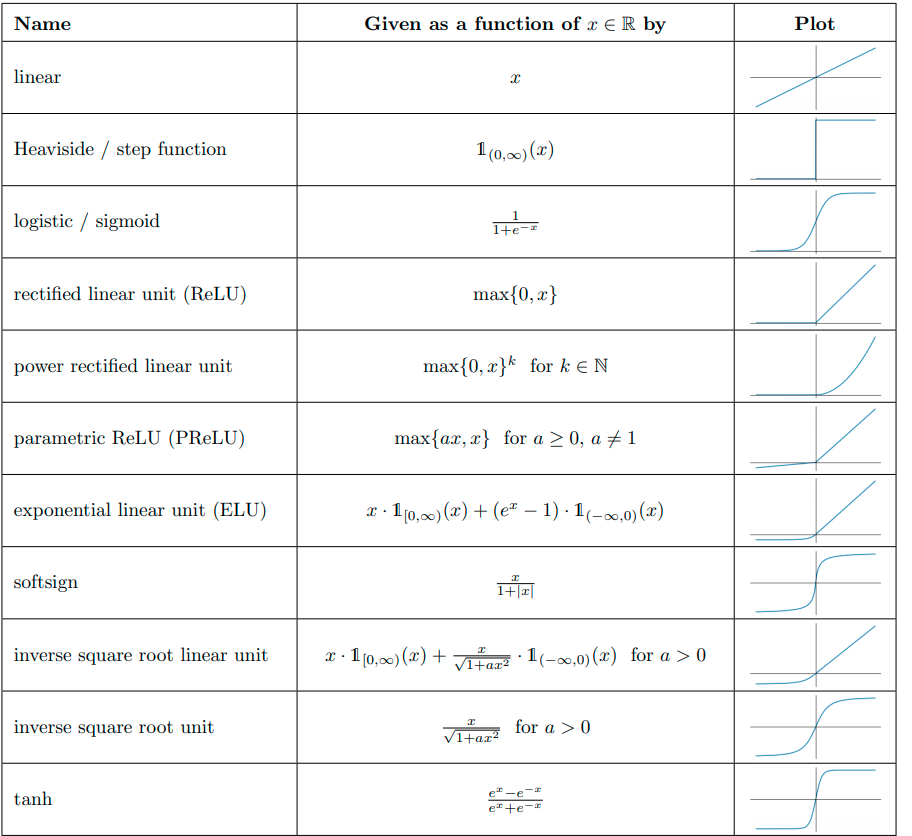
\includegraphics[width=12cm]{latex/figures/activations.png}
    \caption{List of popularly used activation functions for DNNs and other neural networks. The figure is retrieved from \citet{DBLP:journals/corr/abs-2105-04026}.}
    \label{fig:activation function}
\end{figure}

In this thesis, we will be mainly concerned with the activation functions \emph{linear}, \emph{sigmoid} and \emph{tanh}. The linear activation function, or identity function, applies no transformation to the layer output output $\boldsymbol{z} = W^l \boldsymbol{a}^{l-1} + \boldsymbol{b}^l$. This activation function is usually applied to the output layer only, and is useful when we don't want to transform the final output of the DNN into any particular shape. This is usually the case for regression, where the targets we want to predict can be any real value. The sigmoid activation function constraints the output to be in the interval $a^L \in [0, 1]$. This activation is often used on the output layer when doing classification, as the target labels are (in the binary case) $y \in \{0,1\}$. For all hidden layers, we will use tanh activation. This choice is discussed in \cref{sec:Configuring QCNs and DNNs}.

%================================================================
\subsection{Saturated Activations and Vanishing Gradient}\label{sec:Saturated Activations and Vanishing Gradient}
%================================================================

A common problem with many widely used activation functions is \emph{saturation}. An activation function $f(x)$ is said to be saturated when the input $x$ causes it to become locally very flat. From \cref{fig:activation function}, one can see that this happens for the tanh activation for very high or low values of $x$. This causes the derivative of the activation to be approximately zero, i.e. $f'(x) \approx 0$. If sufficiently many activations are saturated in the network, backpropagation \cref{eq:error} tends to produce gradients close to zero. This phenomenon is known as a \emph{vanishing gradient} \cite{shalevshwartz2017failures}, and is known to slow down training of the neural network. Typically, the effect is worse for neural networks with many layers.


%================================================================
\section{Generalizability}\label{sec:Generalizability}
%================================================================
If we obtain a low loss on the training data after fitting a model, can we assume that the resulting model is good and useful? It depends on what we want to use the model for, but if we want to use the model for predicting on new data (data that was not seen during training), we often don't want to train the model too much. As explained earlier, the main goal of a model is to approximate the underlying mechanism $f(\boldsymbol{x})$ of \cref{eq:data} producing the data. If the model fits the data too well, it might also pick up details of the noise $\epsilon$ in the training data, which is called \emph{overfitting}. The problem with this is that if we gather a new data set, a \emph{test set} $y' = f(\boldsymbol{x}) + \epsilon'$, the noise $\epsilon'$ will be different from the noise in the training data because of its random nature. Since the overfitted model is very affected by the noise in the training data, it will likely perform poorly on new data where the noise is different, even though it performs well on the training data. Typically, the more complex and flexible a model is, the more likely it is to overfit the training data. This is because it has a greater capacity to fit the noise present in the training data. By restricting the complexity of the model, one often ends up with a model that resembles $f(\boldsymbol{x})$ more closely. In turn, this results in a model
that \emph{generalizes} better, which means that it makes accurate predictions on values of $\boldsymbol{x}$ not present in the training set. On the other hand, if the model is not complex enough, it might not be sufficiently flexible to recreate $f(\boldsymbol{x})$, causing \emph{underfitting}.

To uncover overfitting, the standard procedure is to prepare independent training and test sets $\mathcal{T}_{Train}$ and $\mathcal{T}_{Test}$, and train the model on the former set and test its performance on the latter. The behaviour of the prediction error, e.g. MSE, on the training and test set is expected to behave as in \cref{fig:train_test}. For models that are optimized iterativly, like neural networks, "model complexity" can be associated with the number of optimization steps. For increasing number of steps, the training error is strictly decreasing, since it is the purpose of training to reduce this quantity. However, the test error has a minimum for which the model shows best generalization. Training beyond this point causes overfitting, increasing the test error. 

\begin{figure}[H]
    \centering
    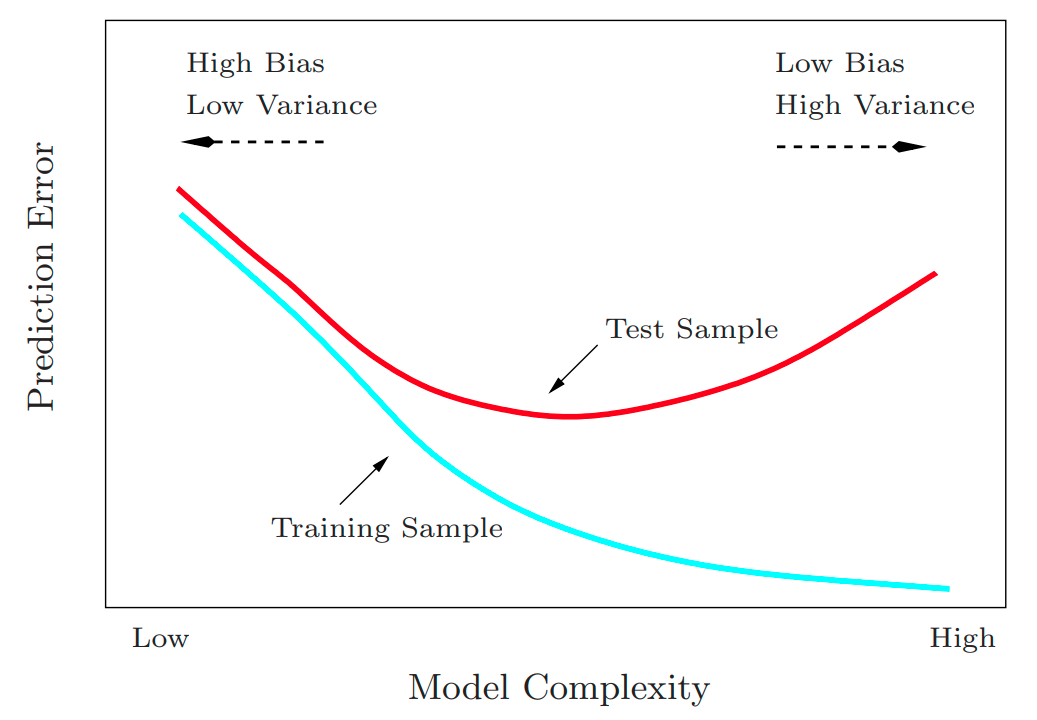
\includegraphics[width=10cm]{latex/figures/train_test.png}
    \caption{Training and test error as a function of model complexity. For models trained iterativly, like neural networks, "Model Complexity" can be associated with the number of optimization steps. The figure is retrieved from \citet{hastie01statisticallearning}.}
    \label{fig:train_test}
\end{figure}


%================================================================
\section{Pre-processing Data}\label{sec:Pre-processing Features Theory}
%================================================================
In this section, we will discuss common techniques for preparing and processing features and data before training models, generally known as \emph{pre-processing}. We start by presenting two methods of scaling features, \emph{standardization} and \emph{min-max scaling}, meant for improving the performance of models. Then, we will present \emph{principal component analysis} (PCA), a technique for reducing the number of features and speeding up training of models. 

%================================================================
\subsection{Scaling Features}\label{sec:Scaling Features}
%================================================================
For data sets gathered for real world applications, it is often the case that the different features have very different units and numerical scales. E.g., a data set detailing health habits may include features such as \emph{age} in the range $0-80$, and \emph{caloric intake} of order $2000$. Many models, such as neural networks, are sensitive to the scales of the features and may perform poorly if they are very different \cite{hands-on}. Therefore, it is typical to scale the features in a way to avoid such outlier values. 

\subsubsection*{Standardization}
For neural networks of the type presented in \cref{sec:DenseNeuralNetwork}, features are often scaled using standardization to improve performance \cite{LeCun2012}. Mathematically, this involves subtracting the mean and divide by the standard deviation over the data set, for each feature:

\begin{equation}
    x_j^{(i)} \rightarrow \frac{x_j^{(i)} - \Bar{x}_j}{\sigma(x_j)},
\end{equation}
where $\Bar{x}_j$ and $\sigma(x_j)$ is the mean and standard deviation of the feature $x_j$, respectively. This ensures that each feature has zero mean and unit standard deviation.

\subsubsection*{Min-Max Scaling}
An alternative to standardization is min-max scaling, useful for when we want the features to lie in a certain interval. To scale the feature $x_j$ to the interval $[a, b]$, we can apply the transformation

\begin{equation}
\begin{aligned}
    x_j^{(i)} \rightarrow (b-a)\frac{x_j^{(i)} - \min(x_j)}{\max(x_j) - \min(x_j)} - a\\
\end{aligned}  
\end{equation}
where $\min(x_j)$ and $\max(x_j)$ return the minimum and maximum value of $x_j$ over the data set, respectively.

%================================================================
\subsection{Principal Component Analysis}\label{sec:Principal Component Analysis}
%================================================================
For data sets with many features, training models may become computationally expensive. Because of this, we often want to reduce the number of features without losing too much of the information of data that may be important for prediction. One way of accomplishing this is with the use of principal component analysis, which applies a linear transformation on the features $x_j$ to derive new features $z_j$ called principal components. The property of the principal components is that they determine the directions in feature space that capture the largest amount of variance in the data, and hence information. The first component $z_1$ is the direction of largest variance, $z_2$ the second largest, etc. In \cref{fig:pca}, the resulting two principal components are visualized for for a data set with two features. For a data set where the features are highly correlated, which is typical for real data sets, performing PCA and keeping the first few components can greatly reduce the number of features without losing too much of the information of the data.

\begin{figure}[H]
    \centering
    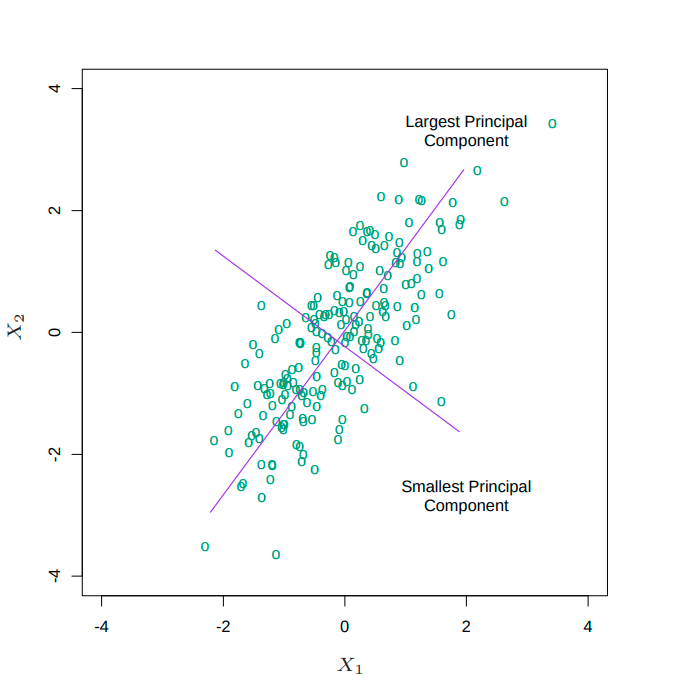
\includegraphics[width=10cm]{latex/figures/pca.png}
    \caption{The two principal components resulting from PCA applied to a data set with two features $x_1$ and $x_2$. The components give the directions in feature space with most and second most variance in the data. The figure is retrieved from \citet{hastie01statisticallearning}.}
    \label{fig:pca}
\end{figure}